\documentclass{article}

\usepackage[printqrbox=false,printhint=false,printanswer=true,printmarkingguide=false,printdraftpaper=false]{unswalgos}

\usepackage{tikz}
\usetikzlibrary{patterns}
\usetikzlibrary{shapes,fit}
\usepackage{tkz-fct}
\usepackage{wrapfig}
\usepackage{subfig}

\usepackage{mathtools}
\usepackage{amssymb}
\usepackage{booktabs,multicol,multirow}
\usepackage{wasysym}
\usepackage{tcolorbox}

\DeclareMathOperator*{\argmax}{arg\,max}
\DeclareMathOperator*{\argmin}{arg\,min}
\DeclareMathOperator{\NAND}{NAND}
\DeclareMathOperator{\AND}{AND}
\DeclareMathOperator{\OR}{OR}
\DeclareMathOperator{\NOT}{NOT}

\usepackage{xspace}

\fancyfoot[L]{\leftmark}
\fancyfoot[R]{\rightmark}

\usepackage{graphicx}
\usepackage{float}
\usepackage{subfigure}

\usepackage{framed}
% This enables new paragraphs without indentation
\usepackage[parfill]{parskip}

\newcommand{\sem}{22T2}
\newcommand{\semester}{Term 2, 2022}
\SubjectNo{COMP3151}
\newcommand{\taskname}{Homework 5}
\Institution{Jinghan Wang, z5286124} % Replace this with your name and zID


\begin{document}

\setcounter{question}{0}

\begin{Question} [\large\textbf {Reasoning about message passing{[5 marks]}}]
Here is a critical section algorithm that uses synchronous message passing:
\begin{figure}[H]
    \centering 
    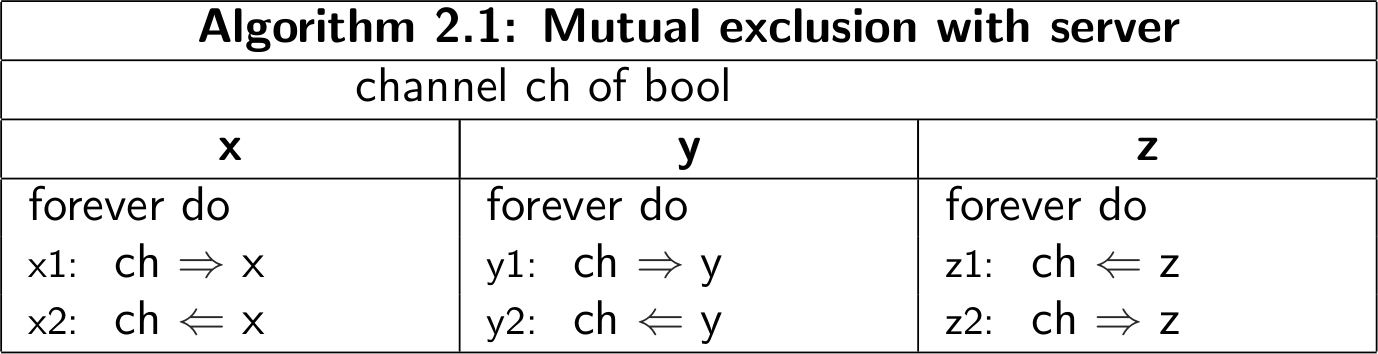
\includegraphics[width=0.8\textwidth]{DV_demand1}
\end{figure}
Only processes $x$ and $y$ are competing for the critical section; $z$ is an auxiliary process. The critical sections are at lines $x2$ and $y2$; $x\_1$ and $y\_1$ are the non-critical sections. The program variables $x,y,z$ are just dummies; their values and types are unimportant.\\\\
The transition diagrams for these processes are as follows.
\begin{figure}[H]
    \centering 
    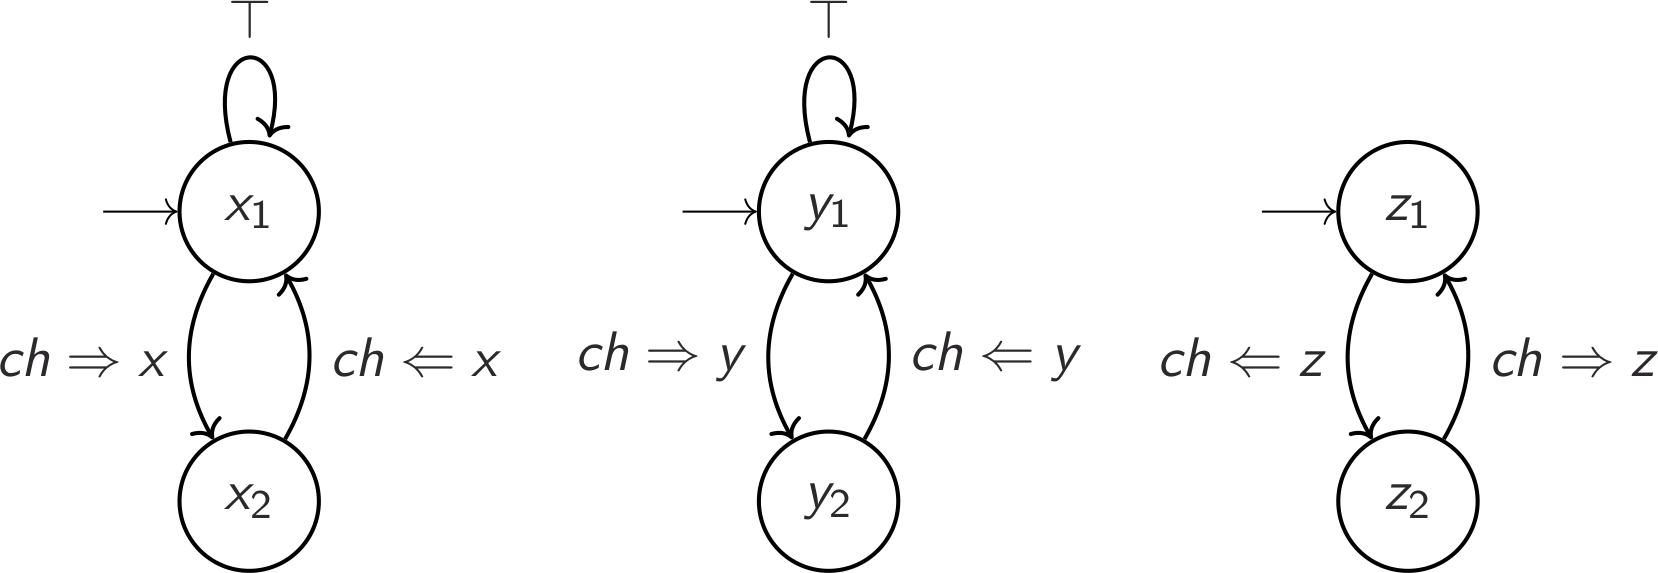
\includegraphics[width=0.8\textwidth]{DV_demand2}
\end{figure}
(The self-loop is not depicted in the code above; it represents the ability to stay in the non-critical section forever).


\begin{Subquestion}
    Construct the closed product of these transition diagrams. The initial state will be $\langle x_1,y_1,z_1 \rangle$.
\begin{answer}
    Answer:
    \begin{figure}[H]
        \centering
        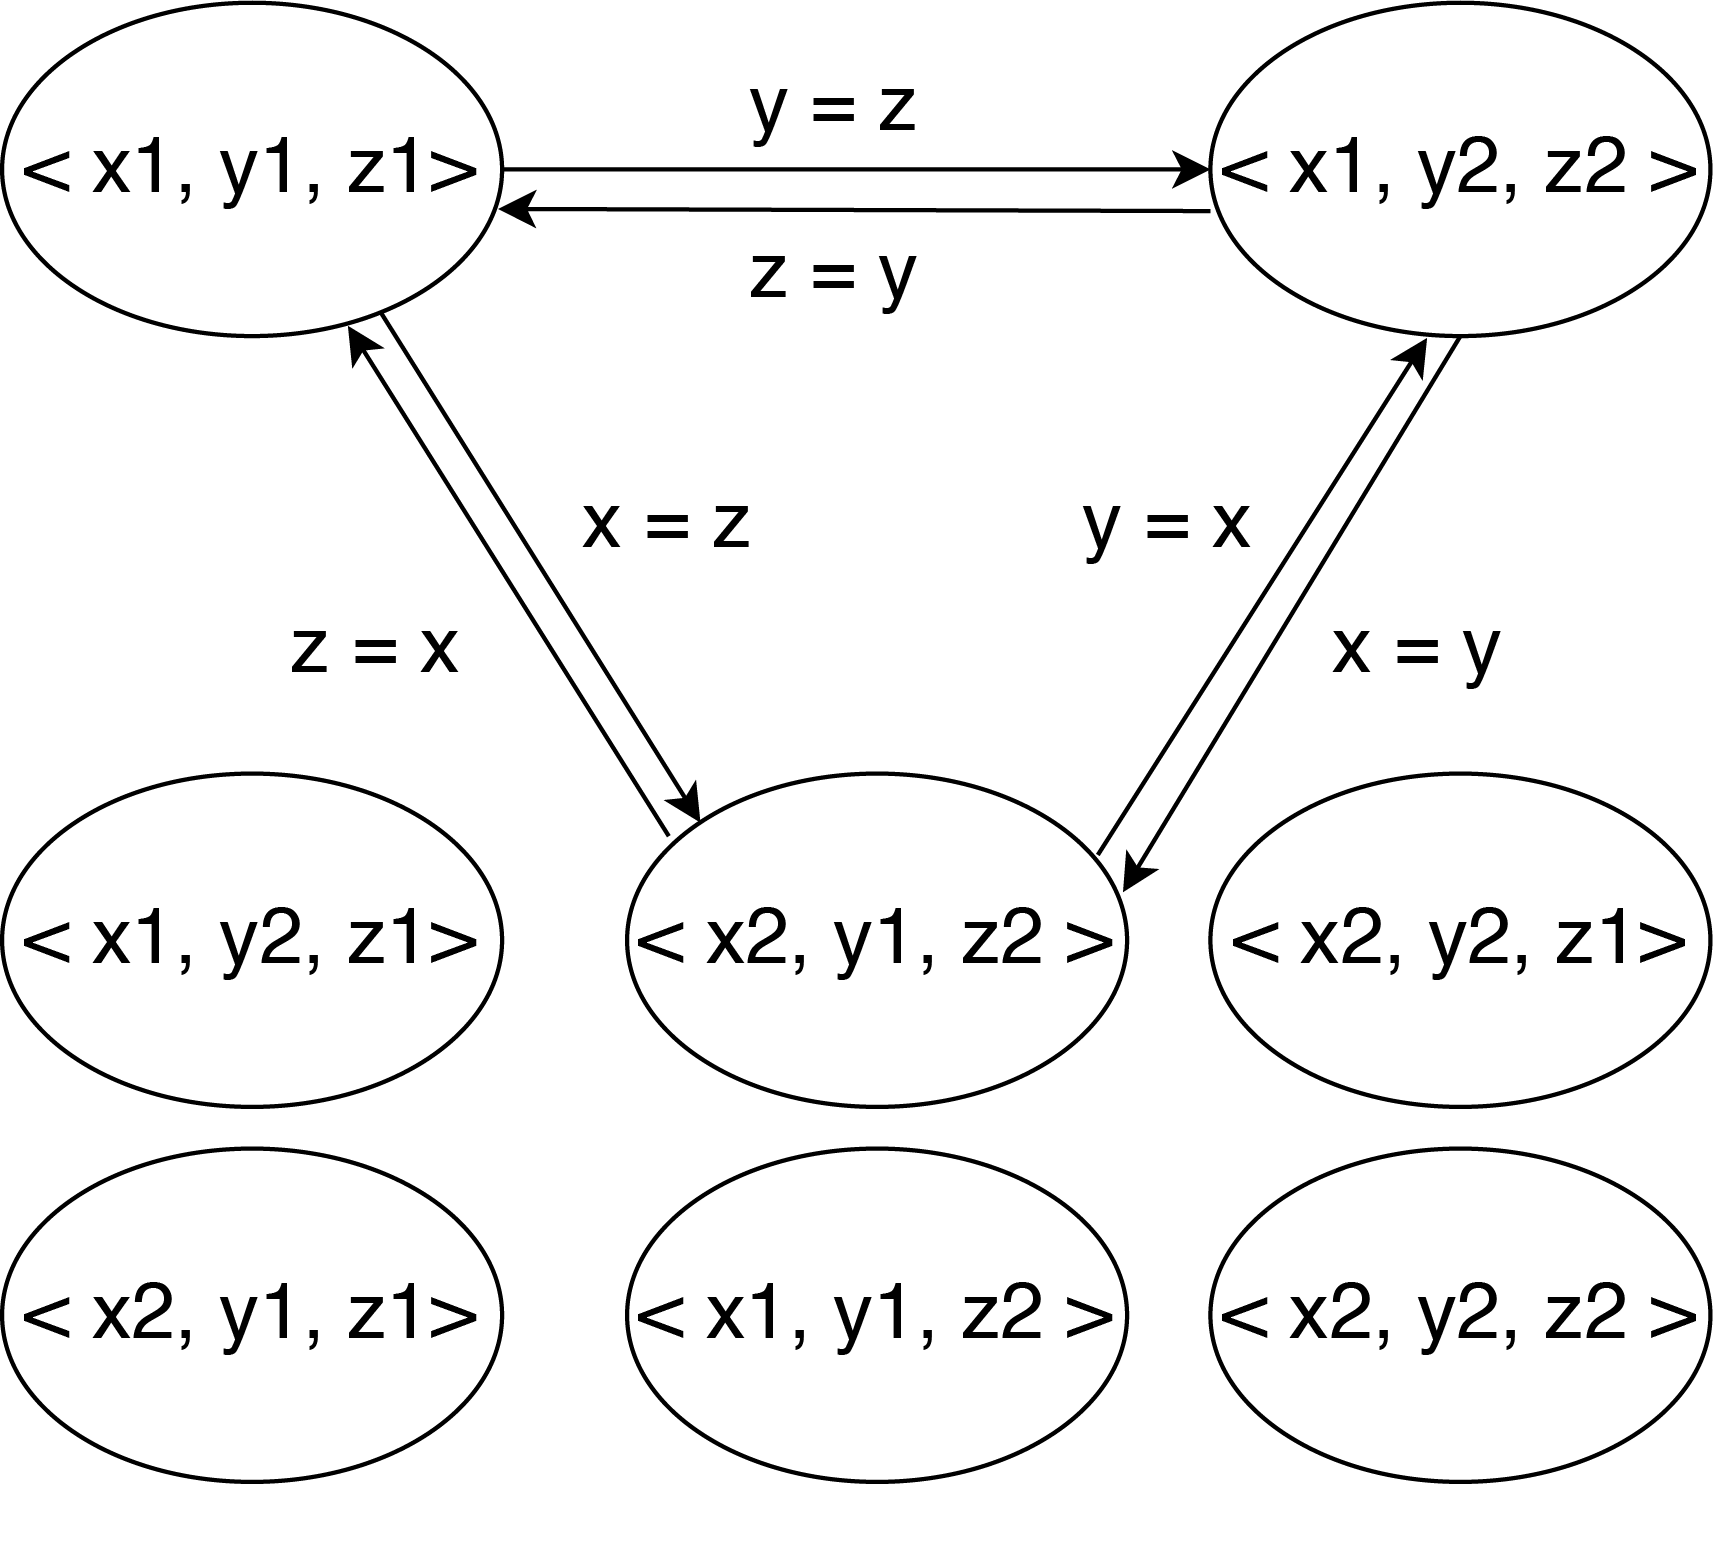
\includegraphics[width=0.48\textwidth]{DV_demand3}
    \end{figure}
\end{answer}
\end{Subquestion}


\begin{Subquestion}
    It's obvious from inspection of the closed product that this algorithm satisfies mutual exclusion. Why?
\begin{answer}
    Answer: 
    
    
\begin{quote}
    \begin{itemize}
        \item[$\bullet$] When $x_1$ is entering in to critical section (ch \Rightarrow x), the $y_1$ and $z_2$ cannot entering.
        \item[$\bullet$] When $y_1$ is entering in to critical section (ch \Rightarrow x), the $x_1$ and $z_2$ cannot entering.
        \item[$\bullet$] When $z_2$ is entering in to critical section (ch \Rightarrow x), the $x_1$ and $y_1$ cannot entering.
    \end{itemize}
    No two processes are in their critical section at the same time. Therefore, it is mutual exclusion.\\
\end{quote}
\end{answer}
\end{Subquestion}


\begin{Subquestion}
    Does this algorithm satisfy eventual entry? Briefly motivate.
\begin{answer}
    Answer:
\begin{quote}
    I don't think so. This may be weak fairness, because if $y_1$ wants to enter the critical section, but it is always preempted by $x_1$ or $z_2$, $y_1$ cannot entry eventual.\\
\end{quote}
\end{answer}
\end{Subquestion}


\begin{Subquestion}
    Does this algorithm still work if we flip all inputs to outputs, and vice versa? Brifely motivate.
\begin{answer}
    Answer: 
\begin{quote}
    No, it's a synchronous channel, when the channel has only input or only output, the input and output are meaningless, because all the input values to the channel and output values from the channel cannot be performed, so the whole algorithm is invalid.\\
\end{quote}
\end{answer}
\end{Subquestion}


\begin{Subquestion}
    The algorithm behaves oddly if we make ch asynchronous. Describe a scenario that (a) assumes an asynchronous, reliable channel; (b) goes on forever in a cycle; and (c) takes transitions other than the self-loops at $x_1$ and $y_1$ infinitely often; and (d) never visits locations $x_2$ and $y_2$.
\begin{answer}
    Answer:
\begin{quote}
    When the channel is asynchronous, input and output are not required at the same time. \\\\
    Therefore, when $z_1$ input does not proceed, $x_1$ and $y_1$ cannot enter the critical section because there is no matching content in the channel. After $z_1$ input, $z_2$ enters the critical section before $x_1$ and $y_1$. $z_1$ input is used by $z_2$ output. When $x_1$ and $y_1$ access the channel again, there is no matching content in channel. When it go back to $z_1$ again, continue the same operation, it matches the situation of the topic.\\
\end{quote}
\end{answer}
\end{Subquestion}
    

\end{Question}
\end{document}